% Options for packages loaded elsewhere
\PassOptionsToPackage{unicode}{hyperref}
\PassOptionsToPackage{hyphens}{url}
%
\documentclass[
]{article}
\usepackage{amsmath,amssymb}
\usepackage{lmodern}
\usepackage{iftex}
\ifPDFTeX
  \usepackage[T1]{fontenc}
  \usepackage[utf8]{inputenc}
  \usepackage{textcomp} % provide euro and other symbols
\else % if luatex or xetex
  \usepackage{unicode-math}
  \defaultfontfeatures{Scale=MatchLowercase}
  \defaultfontfeatures[\rmfamily]{Ligatures=TeX,Scale=1}
\fi
% Use upquote if available, for straight quotes in verbatim environments
\IfFileExists{upquote.sty}{\usepackage{upquote}}{}
\IfFileExists{microtype.sty}{% use microtype if available
  \usepackage[]{microtype}
  \UseMicrotypeSet[protrusion]{basicmath} % disable protrusion for tt fonts
}{}
\makeatletter
\@ifundefined{KOMAClassName}{% if non-KOMA class
  \IfFileExists{parskip.sty}{%
    \usepackage{parskip}
  }{% else
    \setlength{\parindent}{0pt}
    \setlength{\parskip}{6pt plus 2pt minus 1pt}}
}{% if KOMA class
  \KOMAoptions{parskip=half}}
\makeatother
\usepackage{xcolor}
\usepackage[margin=1in]{geometry}
\usepackage{longtable,booktabs,array}
\usepackage{calc} % for calculating minipage widths
% Correct order of tables after \paragraph or \subparagraph
\usepackage{etoolbox}
\makeatletter
\patchcmd\longtable{\par}{\if@noskipsec\mbox{}\fi\par}{}{}
\makeatother
% Allow footnotes in longtable head/foot
\IfFileExists{footnotehyper.sty}{\usepackage{footnotehyper}}{\usepackage{footnote}}
\makesavenoteenv{longtable}
\usepackage{graphicx}
\makeatletter
\def\maxwidth{\ifdim\Gin@nat@width>\linewidth\linewidth\else\Gin@nat@width\fi}
\def\maxheight{\ifdim\Gin@nat@height>\textheight\textheight\else\Gin@nat@height\fi}
\makeatother
% Scale images if necessary, so that they will not overflow the page
% margins by default, and it is still possible to overwrite the defaults
% using explicit options in \includegraphics[width, height, ...]{}
\setkeys{Gin}{width=\maxwidth,height=\maxheight,keepaspectratio}
% Set default figure placement to htbp
\makeatletter
\def\fps@figure{htbp}
\makeatother
\setlength{\emergencystretch}{3em} % prevent overfull lines
\providecommand{\tightlist}{%
  \setlength{\itemsep}{0pt}\setlength{\parskip}{0pt}}
\setcounter{secnumdepth}{-\maxdimen} % remove section numbering
\ifLuaTeX
  \usepackage{selnolig}  % disable illegal ligatures
\fi
\IfFileExists{bookmark.sty}{\usepackage{bookmark}}{\usepackage{hyperref}}
\IfFileExists{xurl.sty}{\usepackage{xurl}}{} % add URL line breaks if available
\urlstyle{same} % disable monospaced font for URLs
\hypersetup{
  pdftitle={Replication Code for Statistical Fallacies in Claims about `Massive and Widespread Fraud' in the 2020 Presidential Election: Examining Claims Based on Aggregate Election Results},
  pdfauthor={Jonathan Cervas; Bernard Grofman},
  hidelinks,
  pdfcreator={LaTeX via pandoc}}

\title{Replication Code for Statistical Fallacies in Claims about
`Massive and Widespread Fraud' in the 2020 Presidential Election:
Examining Claims Based on Aggregate Election Results}
\author{Jonathan Cervas \and Bernard Grofman}
\date{2023-12-05}

\begin{document}
\maketitle

\textbf{Accepted}, \emph{Statistics and Public Policy}

\textbf{In this file, you will find all the code necessary to recreate
any table or figures and other data found in ``Statistical Fallacies in
Claims about `Massive and Widespread Fraud' in the 2020 Presidential
Election: Examining Claims Based on Aggregate Election Results''.}

\begin{center}\rule{0.5\linewidth}{0.5pt}\end{center}

\begin{figure}
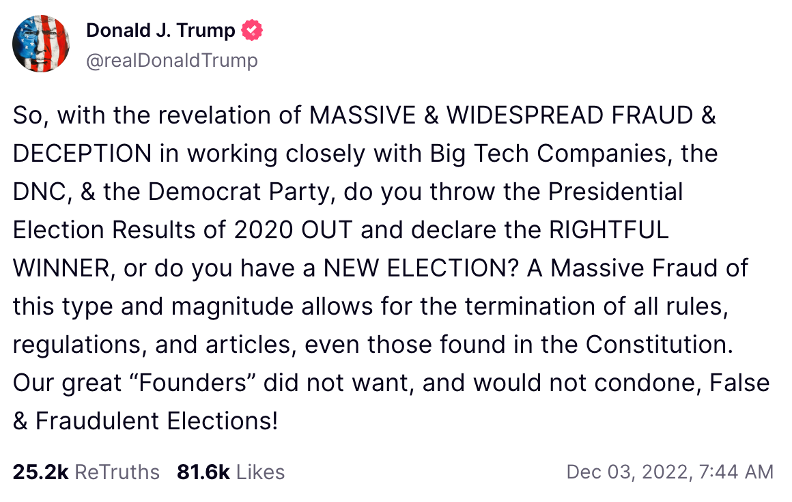
\includegraphics[width=1\linewidth]{images/fig-1-1} \caption{Truth Social post by former President Donald Trump re the lengths he would be prepared to go to overturn the 2020 election results}\label{fig:fig-1}
\end{figure}

\begin{figure}
\centering
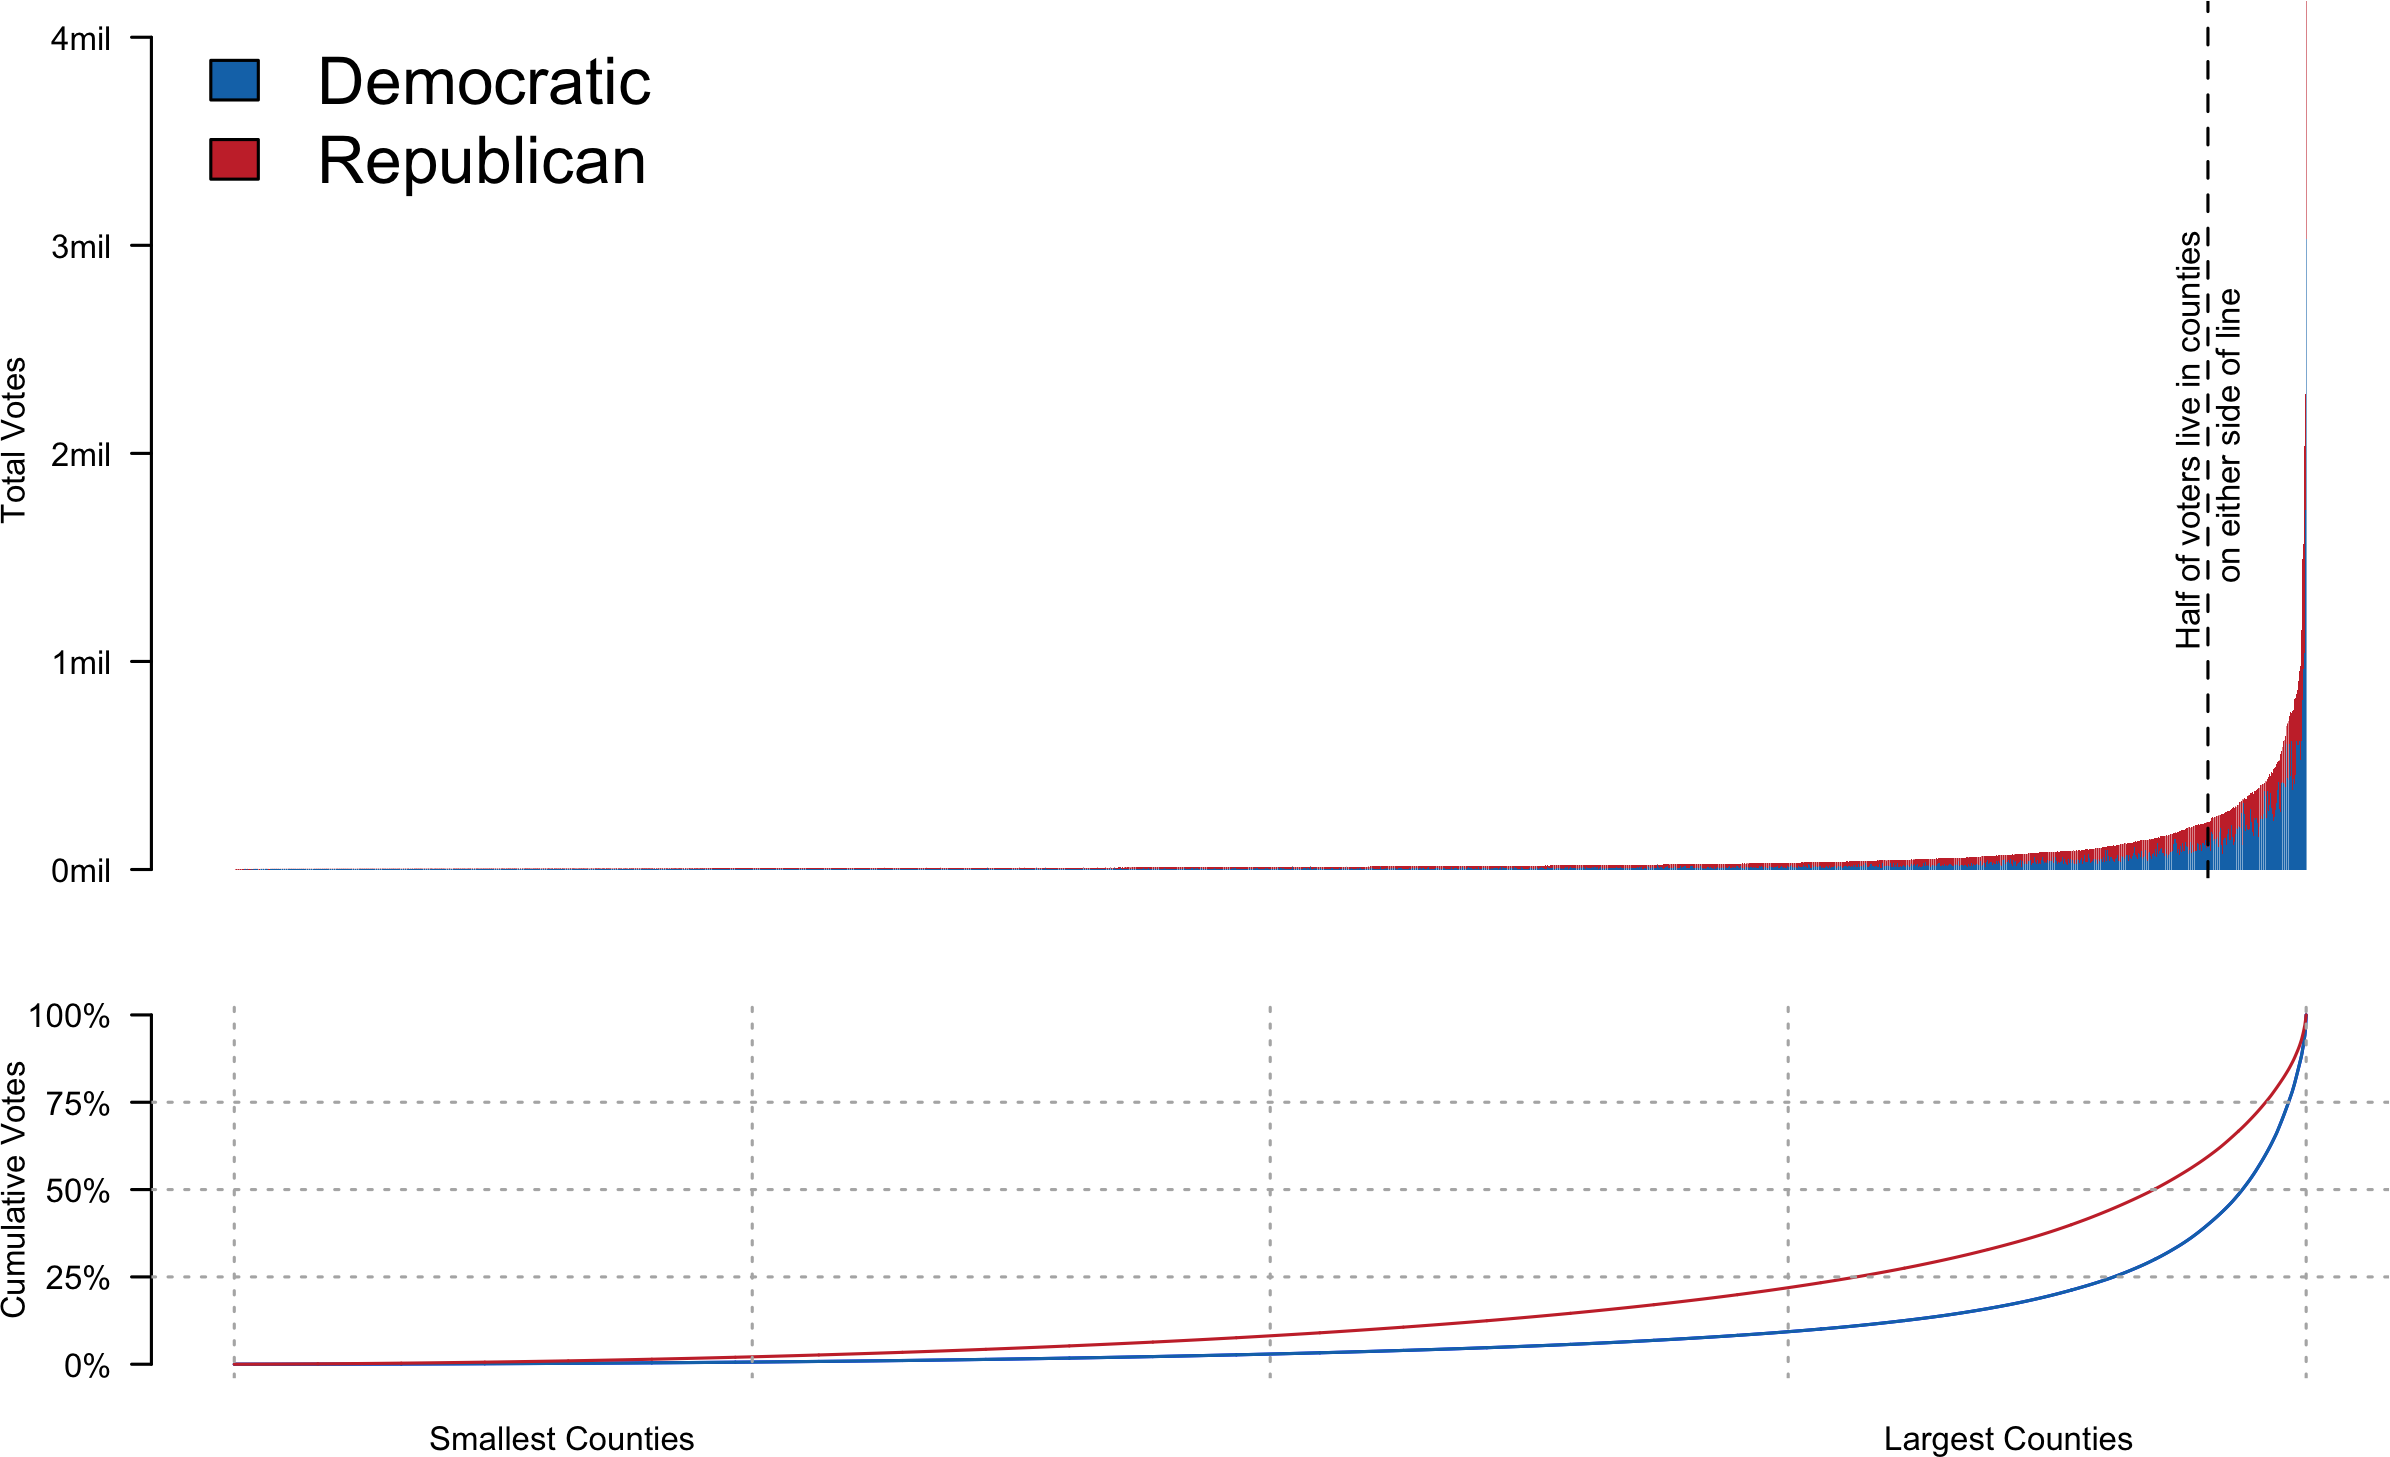
\includegraphics{images/fig-2-1.png}
\caption{Votes in each County}
\end{figure}

\begin{figure}
\centering
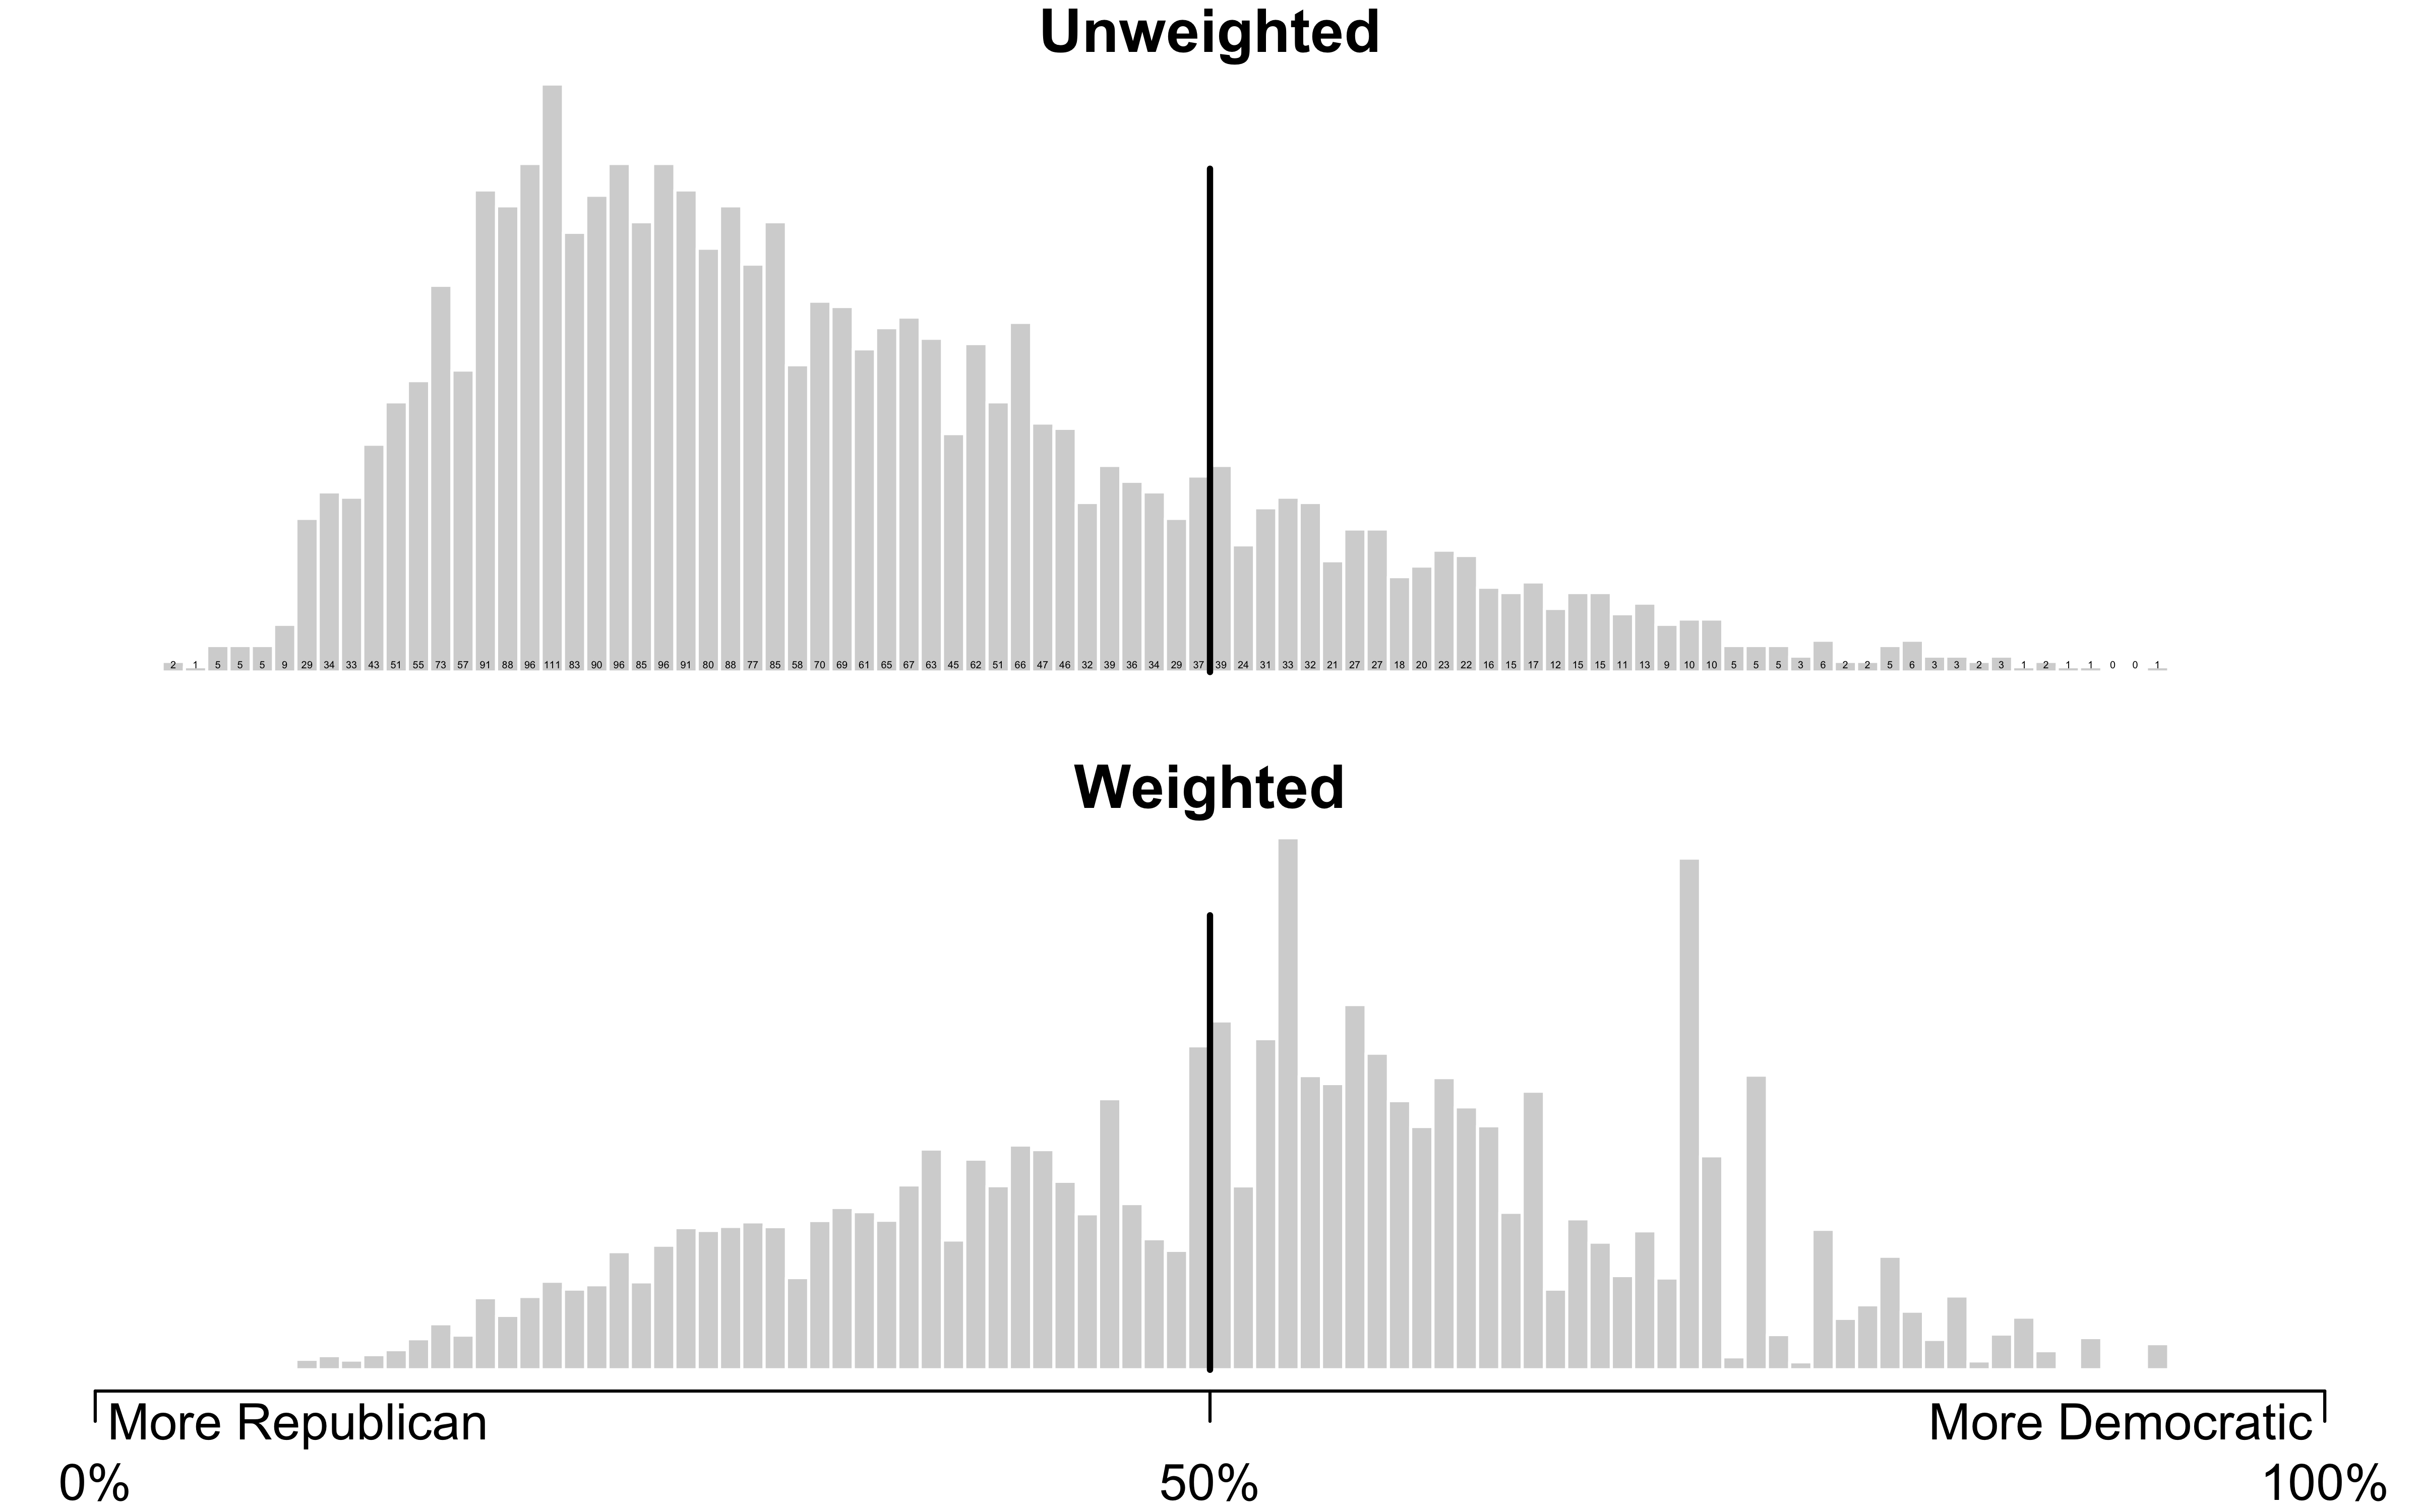
\includegraphics{images/fig-3-1.png}
\caption{Histogram of the 2020 Presidential Election Results, by County}
\end{figure}

\begin{longtable}[]{@{}
  >{\raggedright\arraybackslash}p{(\columnwidth - 2\tabcolsep) * \real{0.9161}}
  >{\raggedright\arraybackslash}p{(\columnwidth - 2\tabcolsep) * \real{0.0839}}@{}}
\caption{Statistical Fallacies Evaluated from the 2020
election}\tabularnewline
\toprule()
\begin{minipage}[b]{\linewidth}\raggedright
Type
\end{minipage} & \begin{minipage}[b]{\linewidth}\raggedright
Examples
\end{minipage} \\
\midrule()
\endfirsthead
\toprule()
\begin{minipage}[b]{\linewidth}\raggedright
Type
\end{minipage} & \begin{minipage}[b]{\linewidth}\raggedright
Examples
\end{minipage} \\
\midrule()
\endhead
Arithmetic Fallacies & Cherry-p\ldots. \\
Misinterpreting Statistical Significance & False Ca\ldots. \\
Meretricious Probabilistic Reasoning & Double V\ldots. \\
Logically Invalid Arguments with a True Premise involving Historical
Election Results Comparisons & Spoiled \ldots. \\
Logically Valid Arguments with a False Premise involving Historical
Election Results Comparisons & Presiden\ldots. \\
Logically Valid Arguments with False Statistical Premises Using
Comparisons Based on Features or Components of the Same Presidential
Election & Split ti\ldots. \\
\bottomrule()
\end{longtable}

\begin{longtable}[]{@{}lrr@{}}
\caption{Popular Vote in Counties Carried by Each
Candidate}\tabularnewline
\toprule()
& Biden Counties & Trump Counties \\
\midrule()
\endfirsthead
\toprule()
& Biden Counties & Trump Counties \\
\midrule()
\endhead
Biden Votes & 59019426 & 22245568 \\
Trump Votes & 33564182 & 40644014 \\
Difference Pro-Trump & -25455244 & 18398446 \\
\bottomrule()
\end{longtable}

\begin{verbatim}
## Registered S3 method overwritten by 'geojsonlint':
##   method         from 
##   print.location dplyr
\end{verbatim}

\begin{longtable}[]{@{}lrrrrr@{}}
\caption{2016 and 2020 Exit Polls, by Race}\tabularnewline
\toprule()
& White & Black & Hispanic & Asian & Other \\
\midrule()
\endfirsthead
\toprule()
& White & Black & Hispanic & Asian & Other \\
\midrule()
\endhead
proportion\_vote & 0.70 & 0.12 & 0.11 & 0.04 & 0.03 \\
Democratic & 0.37 & 0.89 & 0.66 & 0.65 & 0.56 \\
Republican & 0.57 & 0.08 & 0.28 & 0.27 & 0.36 \\
proportion\_vote & 0.67 & 0.13 & 0.13 & 0.04 & 0.04 \\
Democratic & 0.41 & 0.87 & 0.65 & 0.61 & 0.55 \\
Republican & 0.58 & 0.12 & 0.32 & 0.34 & 0.41 \\
\bottomrule()
\end{longtable}

\begin{longtable}[]{@{}lrrr@{}}
\caption{Change in Non-Hispanic White Votes between 2016 and
2020}\tabularnewline
\toprule()
& 2016 & 2020 & Difference \\
\midrule()
\endfirsthead
\toprule()
& 2016 & 2020 & Difference \\
\midrule()
\endhead
Trump & 54531026 & 61565755 & 7034729 \\
Clinton/Biden & 35397332 & 43520620 & 8123287 \\
Other & 5740108 & 1061479 & -4678629 \\
Non-Hispanic White Votes & 95668466 & 106147853 & 10479387 \\
Minority Votes & 41000771 & 52281778 & 11281007 \\
All Votes & 136669237 & 158429631 & 21760394 \\
\bottomrule()
\end{longtable}

\begin{figure}
\centering
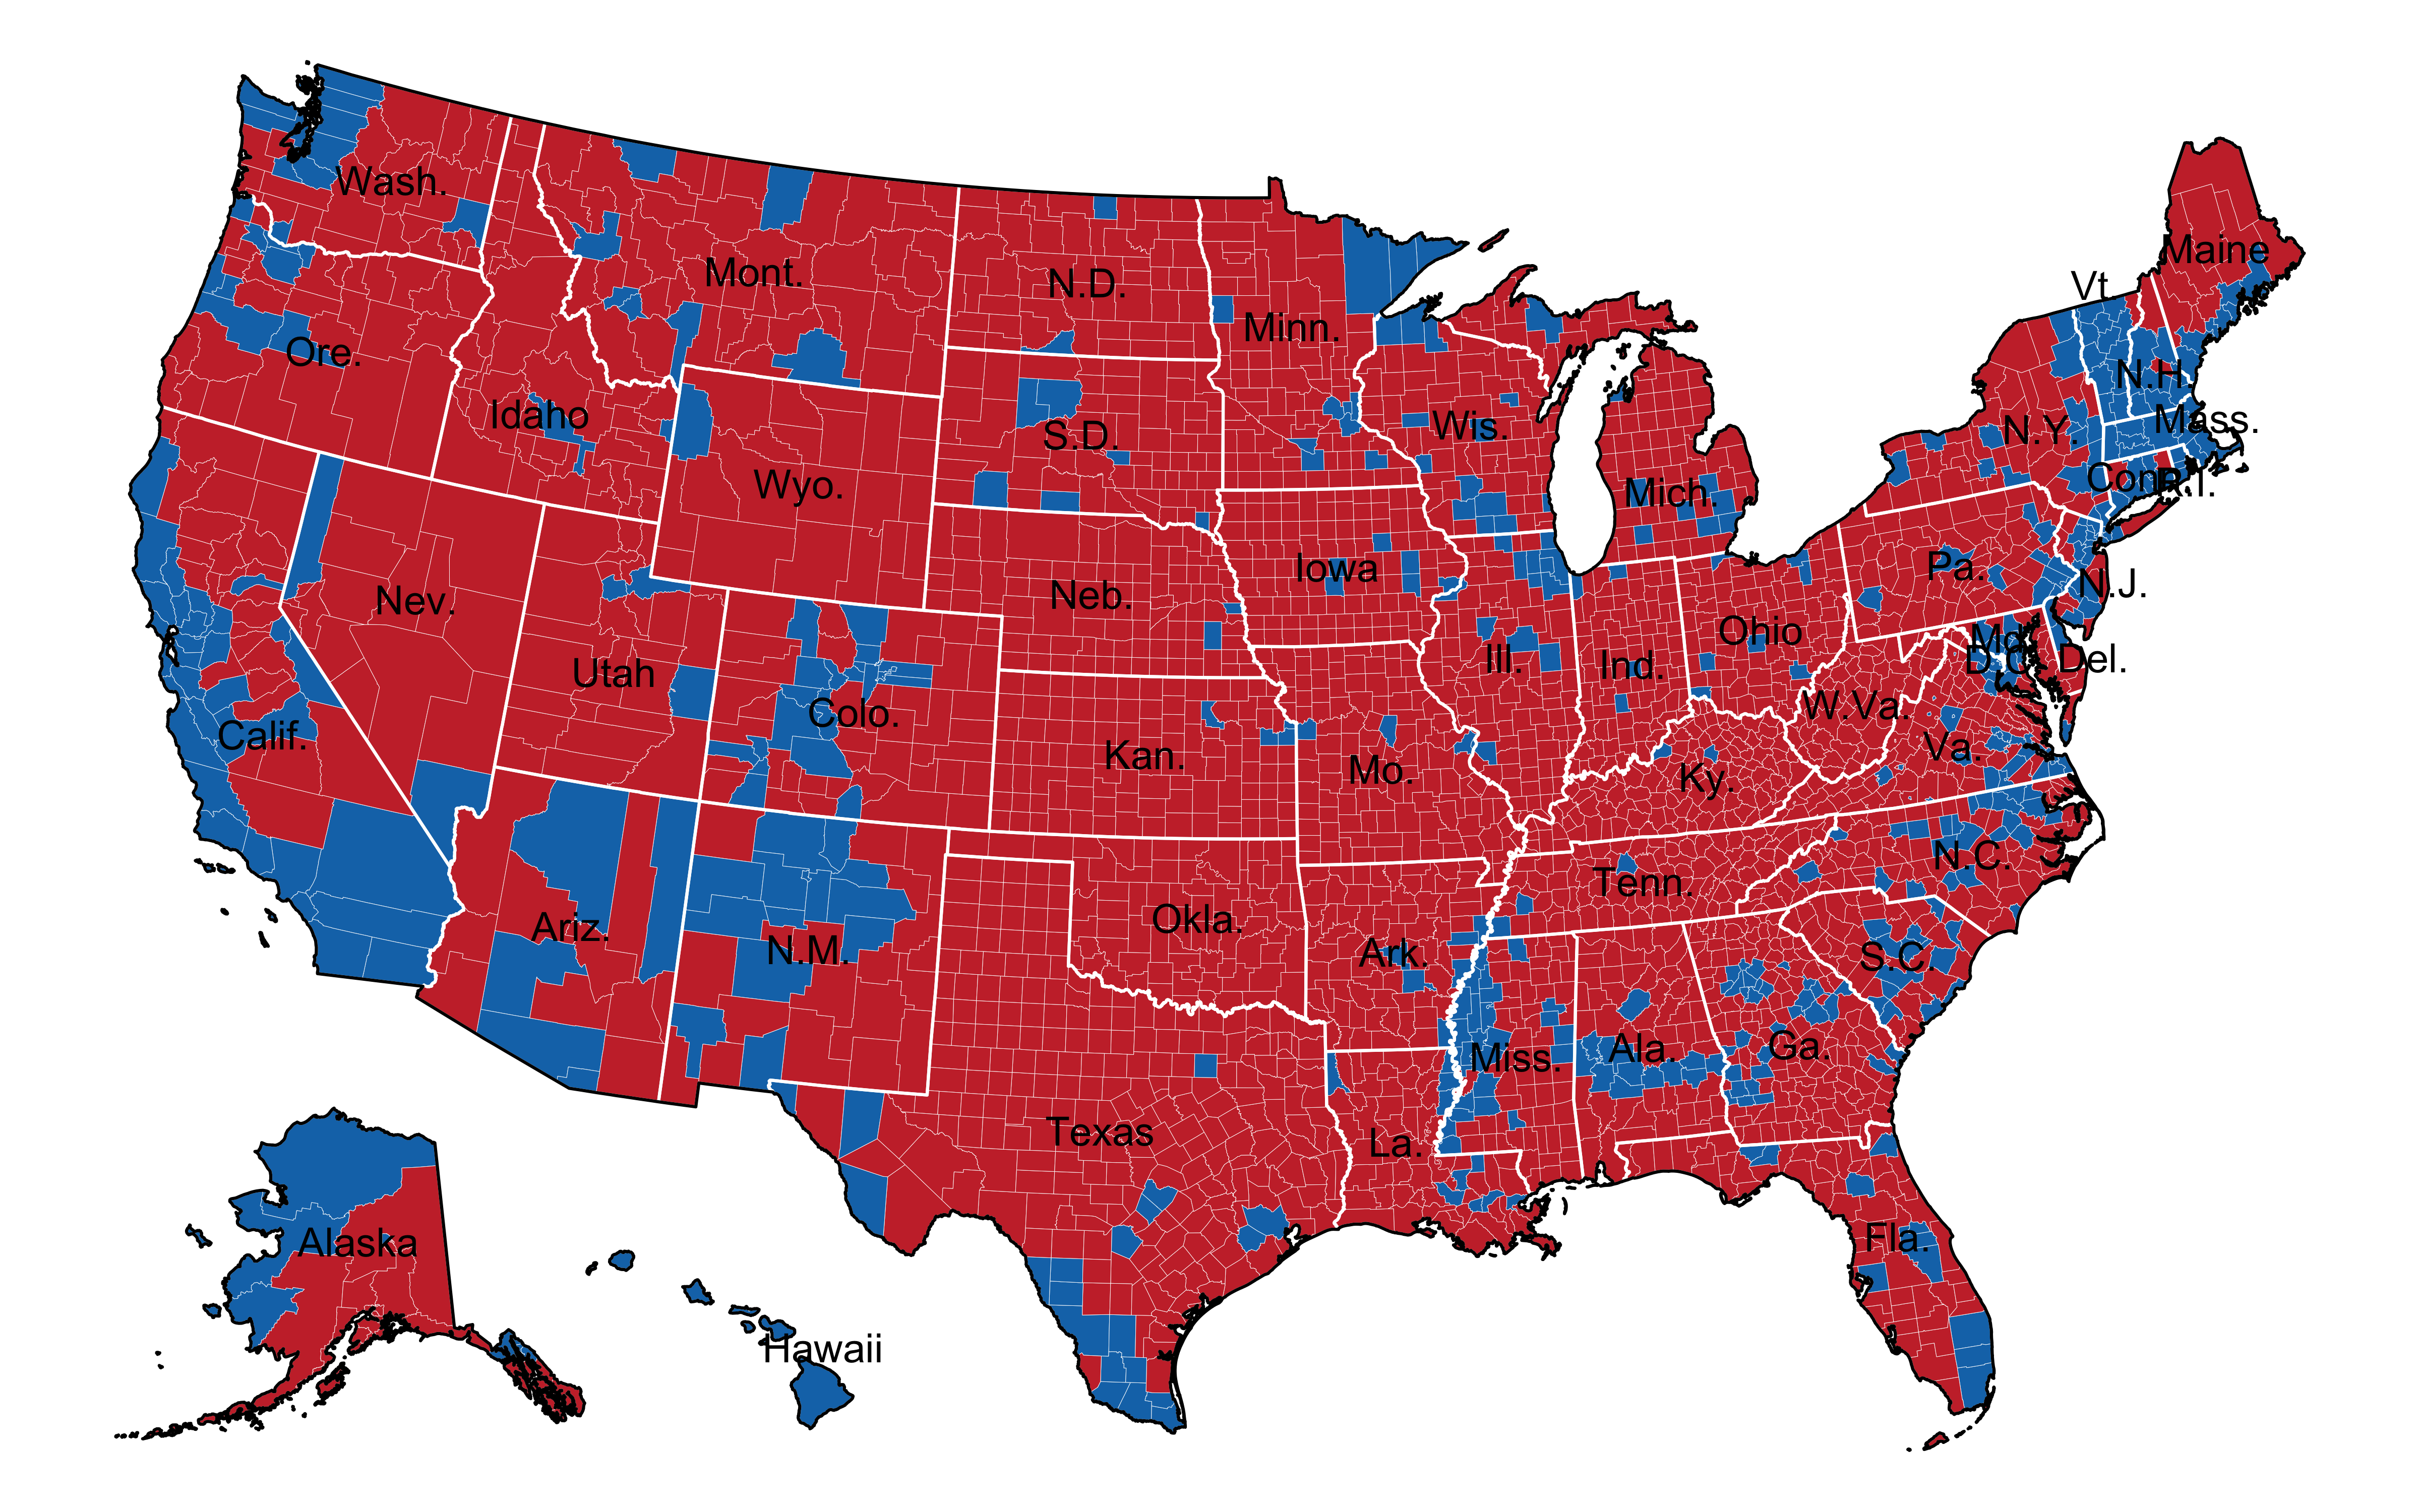
\includegraphics{images/fig-4-1.png}
\caption{Choropleth Plot, 2020 Presidential Election by county}
\end{figure}

\begin{verbatim}
## pdf 
##   2
\end{verbatim}

\begin{figure}
\centering
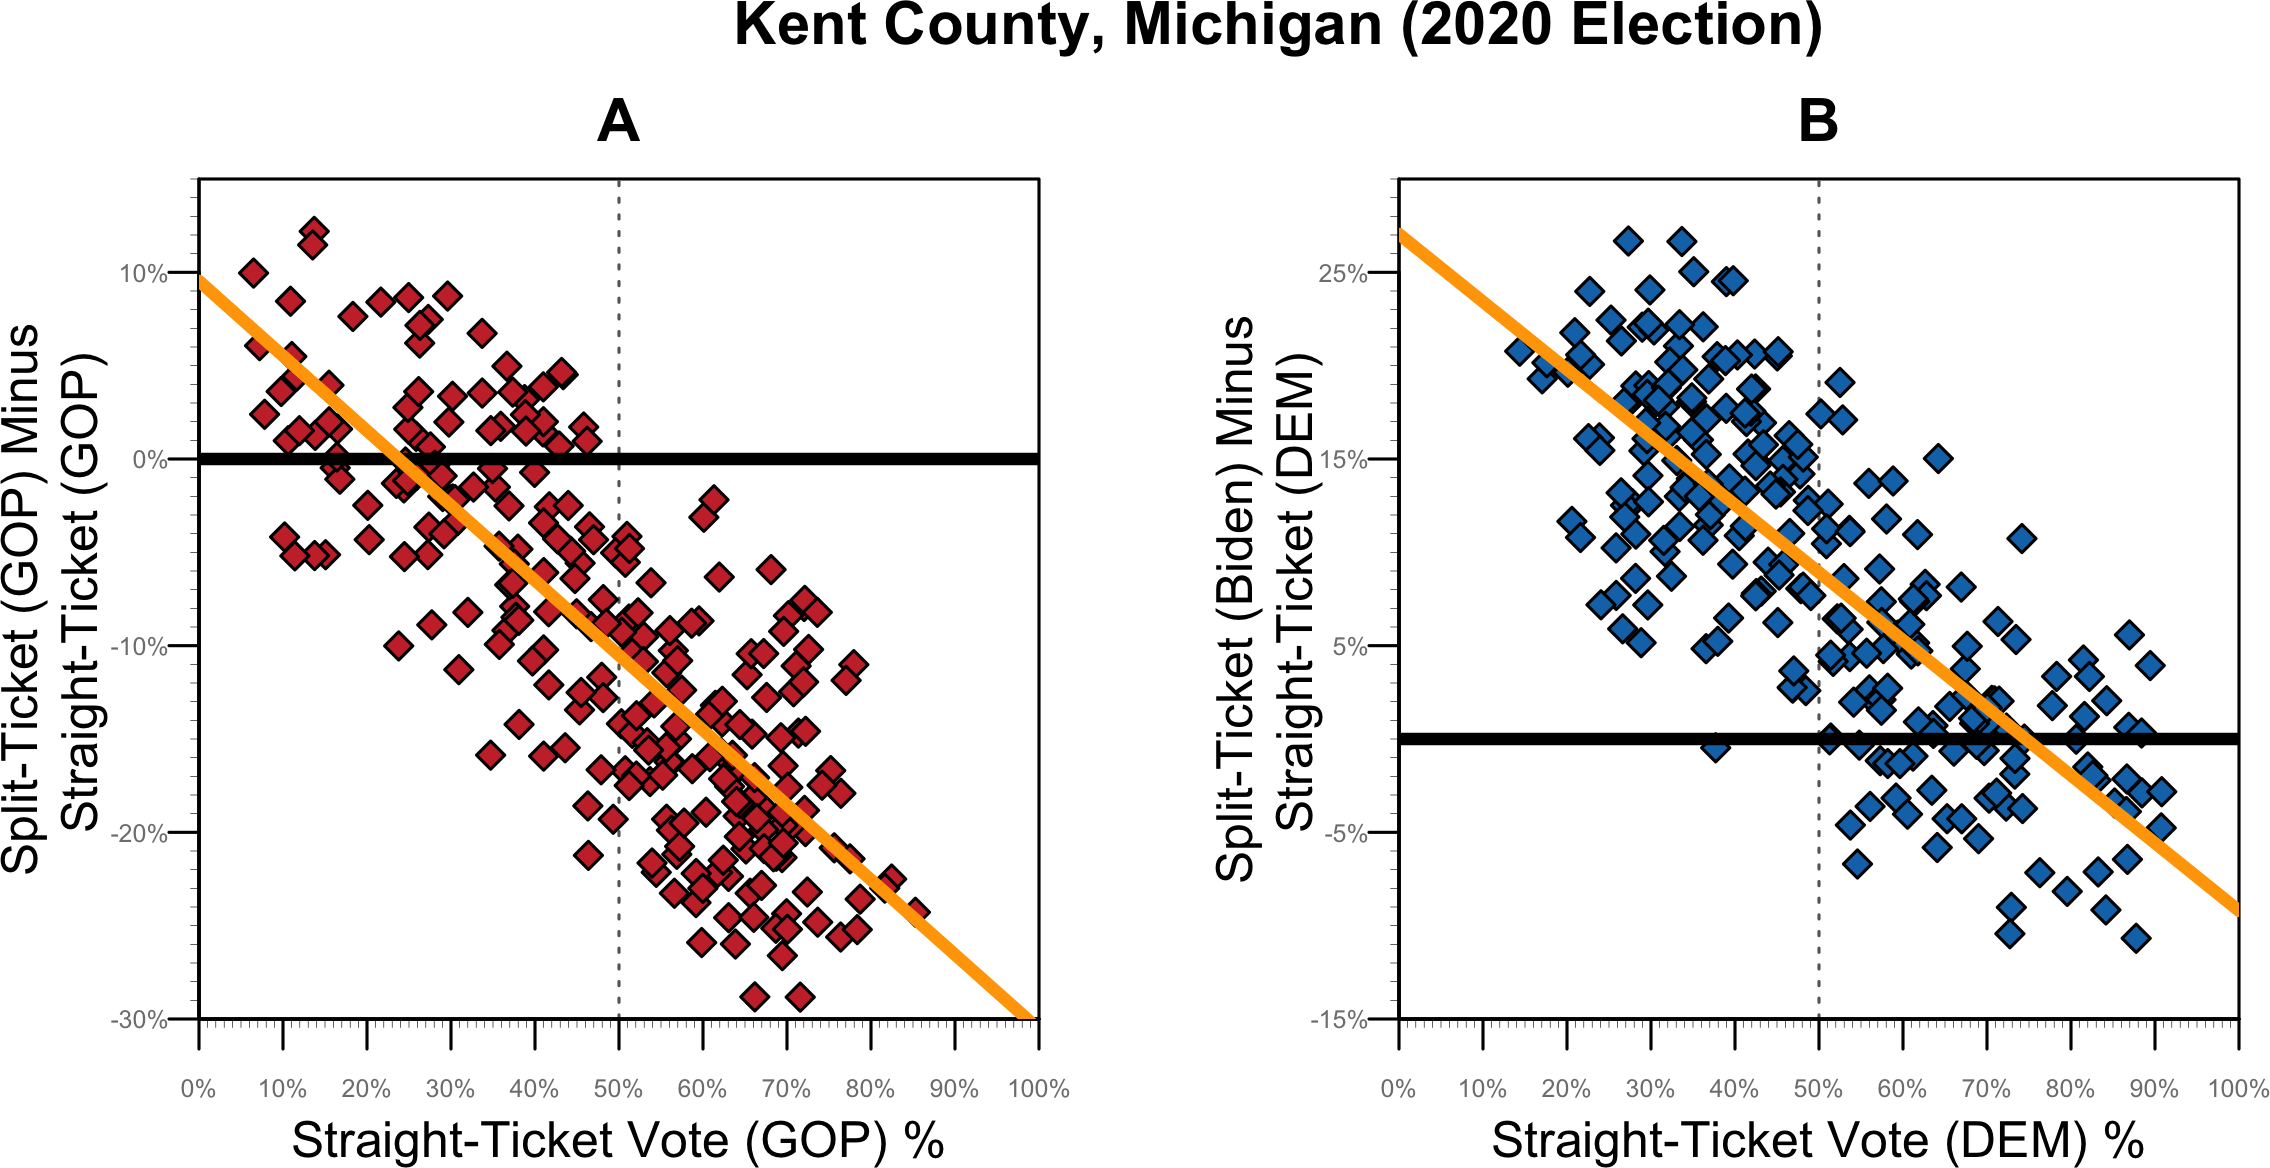
\includegraphics{images/fig-6-1.png}
\caption{Kent County, Michigan 2020 election data plotted as Ayyadurai
shows it}
\end{figure}

\begin{figure}
\centering
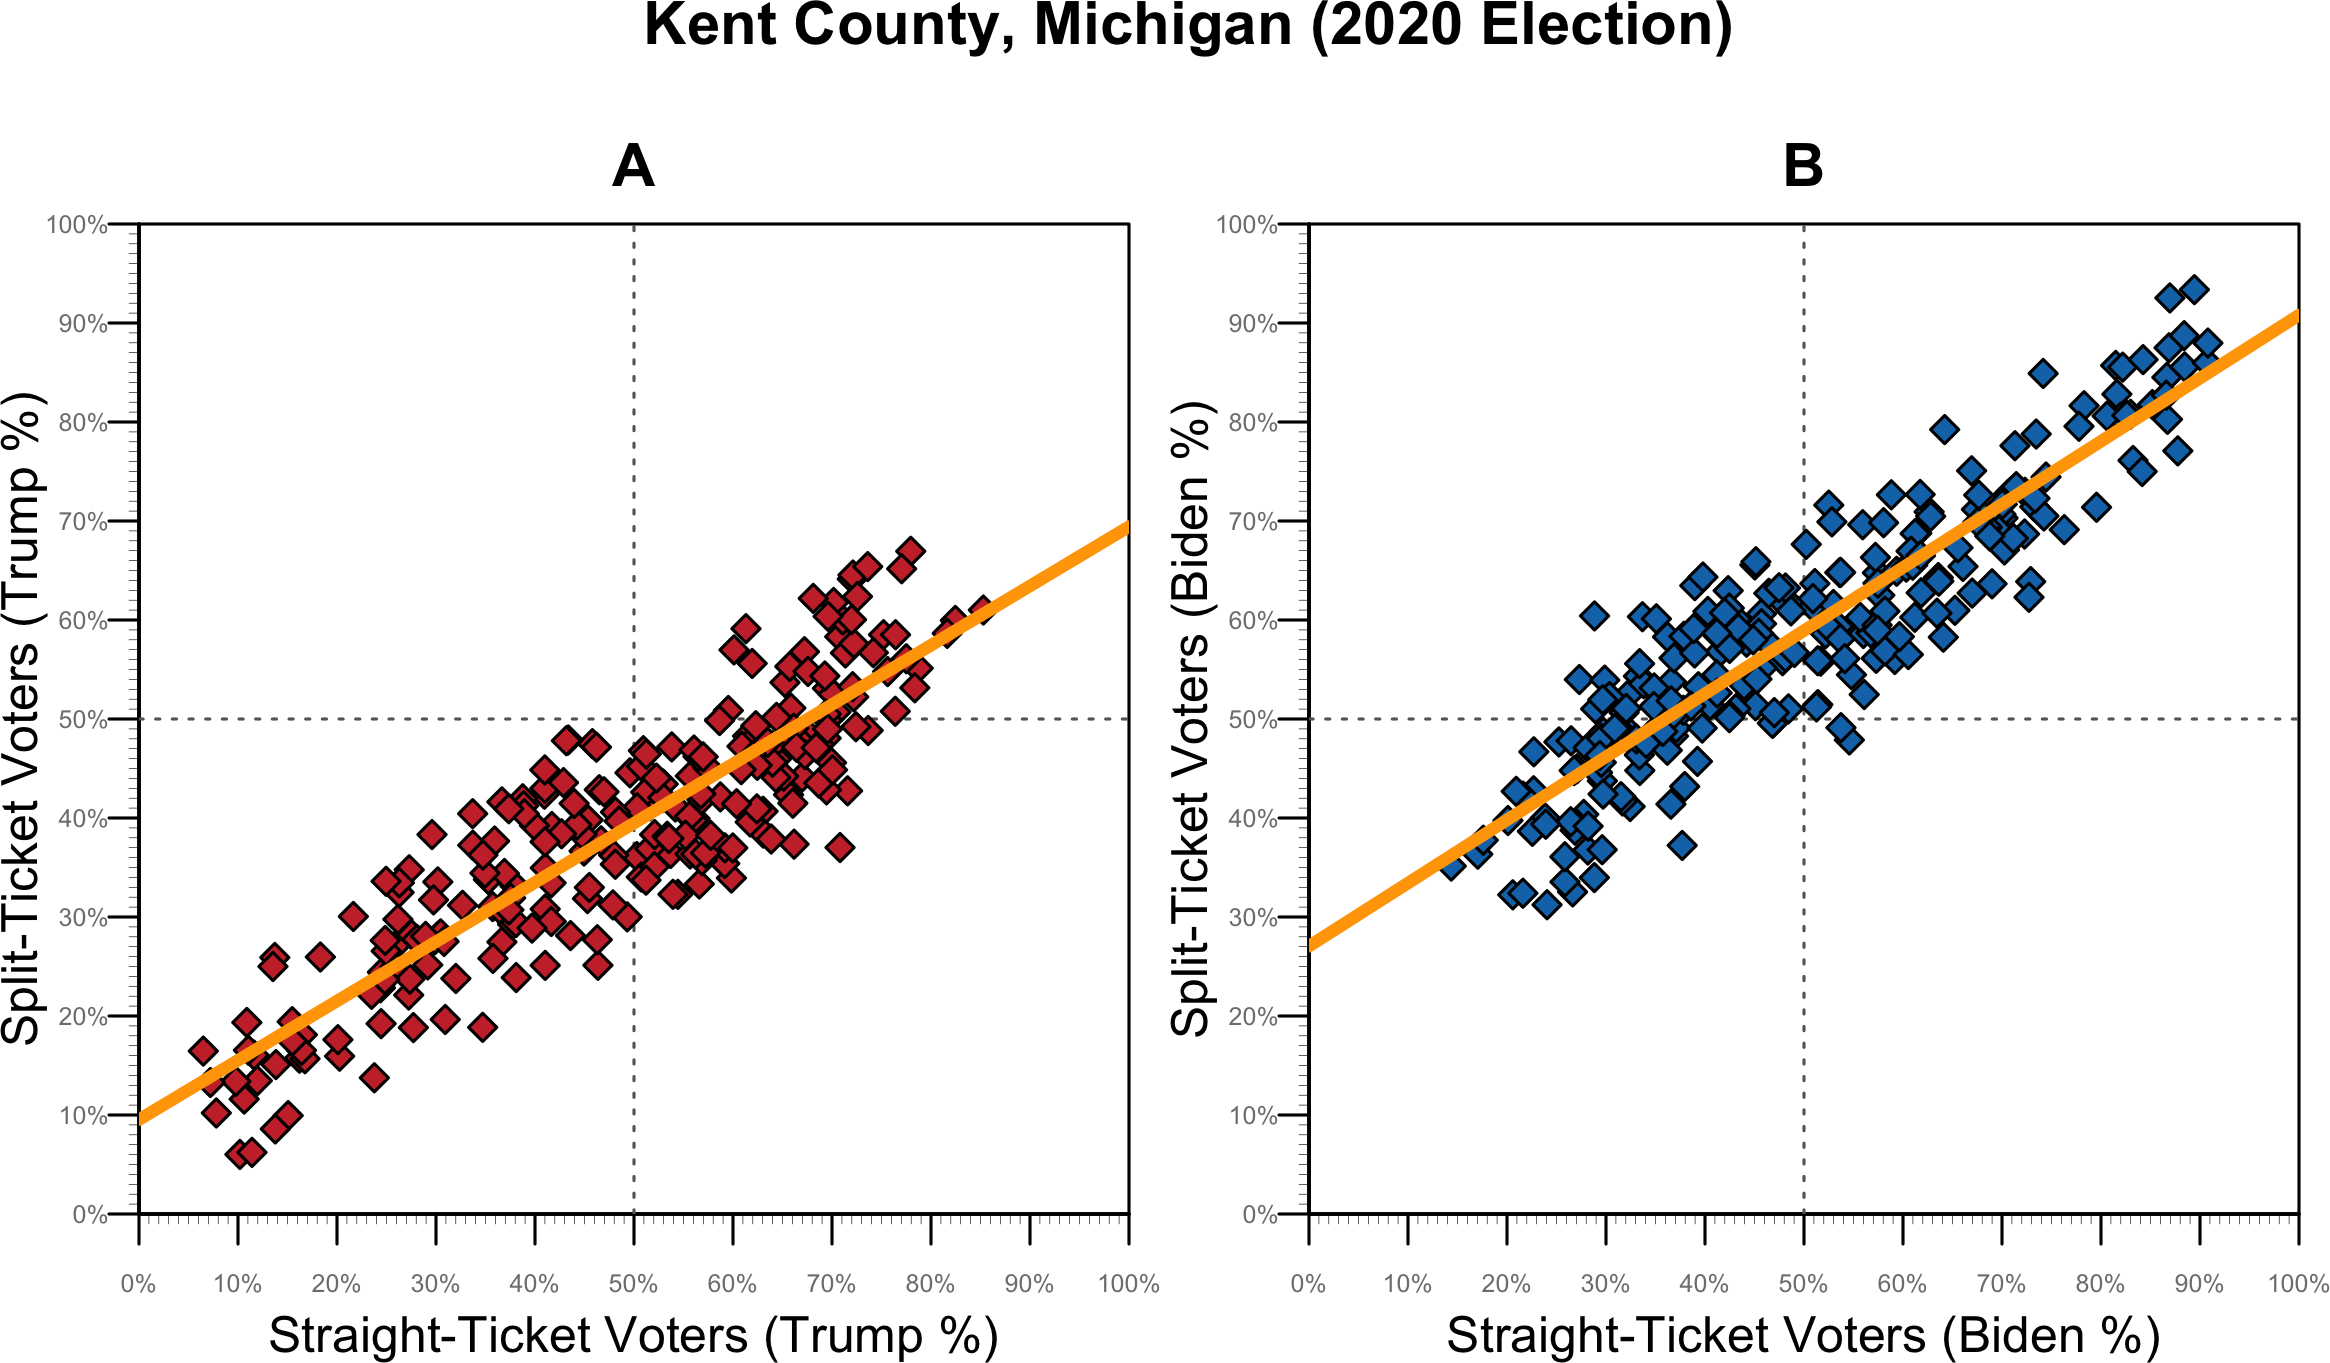
\includegraphics{images/fig-7-1.png}
\caption{Kent County, Michigan Precinct comparison between Trump
Straight-ticket and Trump Split-Ticket Support}
\end{figure}

\end{document}
